% !Mode:: "TeX:UTF-8"

\chapter[tabu算法并行化]{tabu算法并行化}
\section{tabu算法介绍}
tabu算法的核心思想是使用数学优化的局部搜索方法。局部搜索首先选择某个问题的潜在解,然后检查此解的近邻(即类似的
解,只是有微笑的不同)期待获取更好的解决方案.局部搜索方法可能在局部最优的问题上不够理想,但是在许多问题上可以获取
不错的效果。Tabu算法使用特定的数据结果保存已经搜索过的解或者用户自定义的某些规则。如果某个解之前已经使用,
就被标记为"tabu",下次算法将不会再考虑此解。

   kmeans算法核心,如图~\ref{fig:kmeans1}所示,其中黑色点表示待聚类的数据点,红色表示k-means算法实现的分组
情况,蓝色表示每个分组内的中心点

    \begin{figure}[htbp]
    \centering
    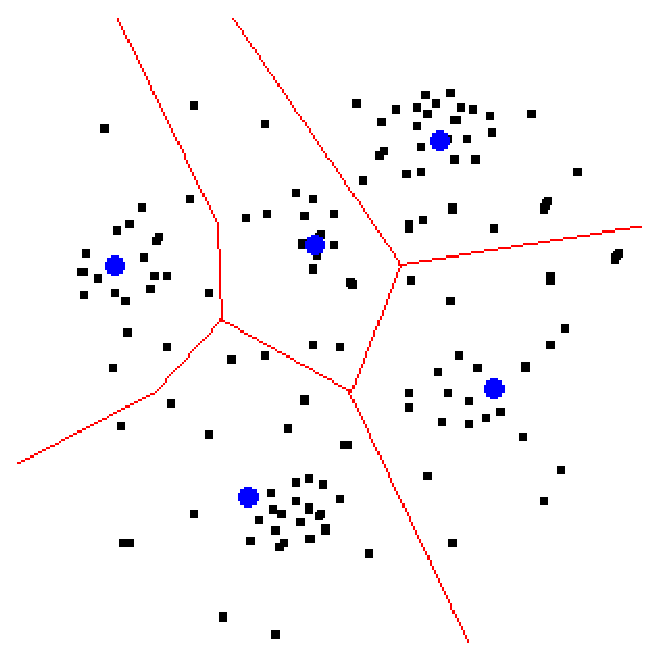
\includegraphics[width=0.4\textwidth]{kmeans1}
    \caption{kmeans}\label{fig:kmeans1}
    \vspace{\baselineskip}
    \end{figure}

\section{算法}

    算法伪代码  

    step1:初始化聚类分组的数目

    step2:初始化分组,确定每个分组的中心点

    step3:对于每个数据点进行以下操作

            step4: 确定当前数据点到每个分组中心点的距离

            step5:对比当前数据点到每个分组中心的距离,将当前数据点归类于距离某个分组中心点距离最小的分组中去

            step6: 更新每个分组的中心,如有变化,跳至step3,当中心点不再发生变化时,跳至step7

    step7:结束整个算法      
            
\section{算法伪代码}

\begin{algorithmic}

\State $s \gets s0$
\State $sBest \gets s$
\State $tabuList \gets null$
\While {$! stopCondition()$}
    \State $candidateList \gets null$ 
    \For {sCandidate in sBeighborhood}
        \If{$!containsTabuElements(sCandidate,tabuList)$}
            \State $candidateList \gets candidateList + sCandidate$
        \EndIf
    \EndFor
    \State $sCandidate \gets LocateBestCandidate(candidateList)$
    \If{$fitness(sCandidate) < fitness(sBest)$}
        \State $tabuList \gets featureDifference(sCandidate,sBest)$
        \State $sBest \gets sCandidate$
        \While{$size(tabuList) > maxTabuListSize$}
            \State ExpireFeatures(tabuList)
        \EndWhile

    \EndIf

\EndWhile    
\State return(sBest)

\end{algorithmic}

\section{实验结果}

%http://en.wikipedia.org/wiki/Tabu_search
